% Options for packages loaded elsewhere
\PassOptionsToPackage{unicode}{hyperref}
\PassOptionsToPackage{hyphens}{url}
%
\documentclass[
  english,
  man,floatsintext]{apa7}
\usepackage{lmodern}
\usepackage{amssymb,amsmath}
\usepackage{ifxetex,ifluatex}
\ifnum 0\ifxetex 1\fi\ifluatex 1\fi=0 % if pdftex
  \usepackage[T1]{fontenc}
  \usepackage[utf8]{inputenc}
  \usepackage{textcomp} % provide euro and other symbols
\else % if luatex or xetex
  \usepackage{unicode-math}
  \defaultfontfeatures{Scale=MatchLowercase}
  \defaultfontfeatures[\rmfamily]{Ligatures=TeX,Scale=1}
\fi
% Use upquote if available, for straight quotes in verbatim environments
\IfFileExists{upquote.sty}{\usepackage{upquote}}{}
\IfFileExists{microtype.sty}{% use microtype if available
  \usepackage[]{microtype}
  \UseMicrotypeSet[protrusion]{basicmath} % disable protrusion for tt fonts
}{}
\makeatletter
\@ifundefined{KOMAClassName}{% if non-KOMA class
  \IfFileExists{parskip.sty}{%
    \usepackage{parskip}
  }{% else
    \setlength{\parindent}{0pt}
    \setlength{\parskip}{6pt plus 2pt minus 1pt}}
}{% if KOMA class
  \KOMAoptions{parskip=half}}
\makeatother
\usepackage{xcolor}
\IfFileExists{xurl.sty}{\usepackage{xurl}}{} % add URL line breaks if available
\IfFileExists{bookmark.sty}{\usepackage{bookmark}}{\usepackage{hyperref}}
\hypersetup{
  pdftitle={Variation in Primary Care Prescribing in Wales due to COVID-19},
  pdflang={en-EN},
  pdfkeywords={keywords},
  hidelinks,
  pdfcreator={LaTeX via pandoc}}
\urlstyle{same} % disable monospaced font for URLs
\usepackage{graphicx,grffile}
\makeatletter
\def\maxwidth{\ifdim\Gin@nat@width>\linewidth\linewidth\else\Gin@nat@width\fi}
\def\maxheight{\ifdim\Gin@nat@height>\textheight\textheight\else\Gin@nat@height\fi}
\makeatother
% Scale images if necessary, so that they will not overflow the page
% margins by default, and it is still possible to overwrite the defaults
% using explicit options in \includegraphics[width, height, ...]{}
\setkeys{Gin}{width=\maxwidth,height=\maxheight,keepaspectratio}
% Set default figure placement to htbp
\makeatletter
\def\fps@figure{htbp}
\makeatother
\setlength{\emergencystretch}{3em} % prevent overfull lines
\providecommand{\tightlist}{%
  \setlength{\itemsep}{0pt}\setlength{\parskip}{0pt}}
\setcounter{secnumdepth}{-\maxdimen} % remove section numbering
% Make \paragraph and \subparagraph free-standing
\ifx\paragraph\undefined\else
  \let\oldparagraph\paragraph
  \renewcommand{\paragraph}[1]{\oldparagraph{#1}\mbox{}}
\fi
\ifx\subparagraph\undefined\else
  \let\oldsubparagraph\subparagraph
  \renewcommand{\subparagraph}[1]{\oldsubparagraph{#1}\mbox{}}
\fi
% Manuscript styling
\usepackage{upgreek}
\captionsetup{font=singlespacing,justification=justified}

% Table formatting
\usepackage{longtable}
\usepackage{lscape}
% \usepackage[counterclockwise]{rotating}   % Landscape page setup for large tables
\usepackage{multirow}		% Table styling
\usepackage{tabularx}		% Control Column width
\usepackage[flushleft]{threeparttable}	% Allows for three part tables with a specified notes section
\usepackage{threeparttablex}            % Lets threeparttable work with longtable

% Create new environments so endfloat can handle them
% \newenvironment{ltable}
%   {\begin{landscape}\begin{center}\begin{threeparttable}}
%   {\end{threeparttable}\end{center}\end{landscape}}
\newenvironment{lltable}{\begin{landscape}\begin{center}\begin{ThreePartTable}}{\end{ThreePartTable}\end{center}\end{landscape}}

% Enables adjusting longtable caption width to table width
% Solution found at http://golatex.de/longtable-mit-caption-so-breit-wie-die-tabelle-t15767.html
\makeatletter
\newcommand\LastLTentrywidth{1em}
\newlength\longtablewidth
\setlength{\longtablewidth}{1in}
\newcommand{\getlongtablewidth}{\begingroup \ifcsname LT@\roman{LT@tables}\endcsname \global\longtablewidth=0pt \renewcommand{\LT@entry}[2]{\global\advance\longtablewidth by ##2\relax\gdef\LastLTentrywidth{##2}}\@nameuse{LT@\roman{LT@tables}} \fi \endgroup}

% \setlength{\parindent}{0.5in}
% \setlength{\parskip}{0pt plus 0pt minus 0pt}

% \usepackage{etoolbox}
\makeatletter
\patchcmd{\HyOrg@maketitle}
  {\section{\normalfont\normalsize\abstractname}}
  {\section*{\normalfont\normalsize\abstractname}}
  {}{\typeout{Failed to patch abstract.}}
\makeatother
\shorttitle{Welsh Primary Care COVID Prescribing}
\author{First Author\textsuperscript{1}\ \& Second Author\textsuperscript{1,2}}
\affiliation{
\vspace{0.5cm}
\textsuperscript{1} Centre for Health Economics \& Medicines Evaluation, Bangor University, LL55 2PZ\\\textsuperscript{2} Institute for the Psychology of Elite Performance, Bangor University, LL55 2PZ}
\authornote{Add complete departmental affiliations for each author here. Each new line herein must be indented, like this line.

Enter author note here.


Correspondence concerning this article should be addressed to First Author, Postal address. E-mail: my@email.com}
\keywords{keywords\newline\indent Word count: X}
\usepackage{lineno}

\linenumbers
\usepackage{csquotes}
\ifxetex
  % Load polyglossia as late as possible: uses bidi with RTL langages (e.g. Hebrew, Arabic)
  \usepackage{polyglossia}
  \setmainlanguage[]{english}
\else
  \usepackage[shorthands=off,main=english]{babel}
\fi

\title{Variation in Primary Care Prescribing in Wales due to COVID-19}

\date{}

\abstract{
One or two sentences providing a \textbf{basic introduction} to the field, comprehensible to a scientist in any discipline.

Two to three sentences of \textbf{more detailed background}, comprehensible to scientists in related disciplines.

One sentence clearly stating the \textbf{general problem} being addressed by this particular study.

One sentence summarizing the main result (with the words ``\textbf{here we show}'' or their equivalent).

Two or three sentences explaining what the \textbf{main result} reveals in direct comparison to what was thought to be the case previously, or how the main result adds to previous knowledge.

One or two sentences to put the results into a more \textbf{general context}.

Two or three sentences to provide a \textbf{broader perspective}, readily comprehensible to a scientist in any discipline.
}

\begin{document}
\maketitle

\hypertarget{methods}{%
\section{Methods}\label{methods}}

\hypertarget{data}{%
\subsection{Data}\label{data}}

\begin{itemize}
\tightlist
\item
  Sources of data

  \begin{itemize}
  \tightlist
  \item
    GP
  \item
    Prescribing
  \item
    QOF
  \item
    WIMD
  \end{itemize}
\item
  Preparing
\end{itemize}

\hypertarget{identifying-changes-in-prescribing-due-to-covid-19}{%
\subsection{Identifying changes in prescribing due to COVID-19}\label{identifying-changes-in-prescribing-due-to-covid-19}}

Identifying the effects of COVID-19 is not simple, as its effects are unprecedented and its global impact prevents us from adopting a traditional treatment and control group type design. Instead, we have used time series analysis methods to create counterfactual forecasts

To understand the changes in levels of prescribing due to COVID-19, it was first necessary for us to forecast the levels of prescribing had COVID-19 not affected Wales as a baseline. To do so, we used historic data (January 2015 to December 2020) to identify from a range of time series models, one that was good fit to the data. This was done using cross-validation to reduce the likelihood of choosing a model that was overfitted to the data.

\begin{itemize}
\item
  Given the presence of seasonal variation and existing trends in levels of prescribing, we used various time series forecasting methods to account for existing trends and seasonal variation when creating the forecasts.
\item
  For each analysis, we created a forecast that aimed to answer the question, \enquote{What would the levels of prescribing have been if COVID-19 had not affected Wales?} We then used these forecasts to estimate the changes in levels of prescribing due to COVID-19.

  \begin{itemize}
  \tightlist
  \item
    We viewed this, somewhat complex, approach as superior to more simple approaches (e.g., carrying last years levels forward, or even using the mean of the last three years).
  \end{itemize}
\item
  We did not assume that the existing processes would be the same for all drugs or all GP practices, therefore, we investigated the fit of several different time series models to the pre-COVID data.

  \begin{itemize}
  \tightlist
  \item
    Using Jan 2015 to Feb 2020 data, we fitted several different models and assessed their accuracy using a cross-validated process to reduce the likelihood of overfitting models to the data.

    \begin{itemize}
    \item
      Started with 36 months of data, used 6-month horizon as this was the horizon we would be using for the forecasts, 3-month step (to reduce computation time) \textbf{Do we want to re-run this with 1-month?}
    \item
      Only interested in one forecast horizon: six-months
    \item
    \end{itemize}
  \item
    Having chosen the \enquote{best model} for each practice based on the pre-COVID data, we then used this to forecast the level of prescribing for each practice
  \end{itemize}
\item
  We used time series modelling to forecast Welsh primary care prescribing levels had .

  \begin{itemize}
  \tightlist
  \item
    We used the \texttt{fable} (O'Hara-Wild et al., 2021a), \texttt{fasster} (O'Hara-Wild \& Hyndman, 2021), and the \texttt{fable.prophet} (O'Hara-Wild, 2020) packages to conduct the time series analyses.
  \item
    Time series linear model
  \item
    Decomposition model
  \item
    Seasonal naïve (with and without drift)
  \item
    Autoregressive integrated moving average (ARIMA; Box et al., 2015)
  \item
    Holt-Winters Additive Model (Chatfield, 1978)
  \item
    Prophet (Taylor \& Letham, 2018)
  \item
    Combination models (cf.~Thomson et al., 2019)
  \item
    Prescribing quantities log transformed and forecasts use median values to reduce bias that back transformation would introduce when using the mean
  \item
    Model selection

    \begin{itemize}
    \tightlist
    \item
      Ranked by RMSE and Winkler ({\textbf{???}}), then the best mean ranking model is chosen

      \begin{itemize}
      \tightlist
      \item
        Winkler score penalises models that have observations falling outside the prediction interval, thus rewards models with narrow intervals
      \end{itemize}
    \item
      This combination accounts for both the point and distributional accuracy of the forecasts
    \end{itemize}
  \end{itemize}
\end{itemize}

\hypertarget{identifying-different-prescribing-behaviours---lpa}{%
\subsection{Identifying different prescribing behaviours - LPA}\label{identifying-different-prescribing-behaviours---lpa}}

\begin{itemize}
\tightlist
\item
  What is LPA

  \begin{itemize}
  \tightlist
  \item
    Differences from clustering methods (e.g., k-means and hierarchical)
  \end{itemize}
\end{itemize}

When conducting LPA, several models are specified and then evaluated. Model selection, including class enumeration, should not be based solely on statistical criteria, but also the statistical adequacy and substantive meaning of the solutions ({\textbf{???}}; Marsh et al., 2009). Indeed, relying solely on statistical criteria in large samples may lead to the inability to identify an \enquote{optimal solution} as model fit increases as the number of classes increase ({\textbf{???}}).

In this study we inspected the Bayesian Information Criterion (BIC; Schwartz, 1978) and the bootstrapped likelihood ratio test (BLRT; McLachlan \& Peel, 2000) during the class enumeration process as the results of Monte-Carlo simulation study (Nylund et al., 2007) showed them outperform other information criteria and likelihood-based tests.

\begin{itemize}
\tightlist
\item
  Entropy
\item
  Posterior probabilities
\end{itemize}

\hypertarget{reproducability-and-code}{%
\subsection{Reproducability and code}\label{reproducability-and-code}}

We used R (Version 4.0.2; R Core Team, 2020) and the R-packages \emph{dplyr} (Version 1.0.4; Wickham, François, et al., 2021), \emph{fable} (Version 0.3.0; O'Hara-Wild et al., 2021a, 2021b; O'Hara-Wild, 2020), \emph{fable.prophet} (Version 0.1.0; O'Hara-Wild, 2020), \emph{fabletools} (Version 0.3.0; O'Hara-Wild et al., 2021b), \emph{fasster} (Version 0.1.0.9100; O'Hara-Wild \& Hyndman, 2021), \emph{feasts} (Version 0.1.7; O'Hara-Wild et al., 2021c), \emph{forcats} (Version 0.5.1; Wickham, 2021), \emph{furrr} (Version 0.2.2; Vaughan \& Dancho, 2021), \emph{future} (Version 1.21.0; Bengtsson, 2020), \emph{ggplot2} (Version 3.3.3; Wickham, 2016), \emph{lubridate} (Version 1.7.10; Grolemund \& Wickham, 2011), \emph{MplusAutomation} (Version 0.8; Hallquist \& Wiley, 2018), \emph{papaja} (Version 0.1.0.9942; Aust \& Barth, 2020), \emph{prophet} (Version 0.6.1; O'Hara-Wild, 2020; Taylor \& Letham, 2020), \emph{purrr} (Version 0.3.4; Henry \& Wickham, 2020a), \emph{Rcpp} (Version 1.0.6; Eddelbuettel \& François, 2011; Eddelbuettel \& Balamuta, 2018), \emph{readr} (Version 1.4.0; Wickham \& Hester, 2020), \emph{rebus} (Version 0.1.3; Cotton, 2017), \emph{rlang} (Version 0.4.10; Henry \& Wickham, 2020b), \emph{rstan} (Version 2.21.2; Stan Development Team, 2020a), \emph{serCymruTools} (Version 0.1.3; Will, 2021), \emph{StanHeaders} (Version 2.21.0.7; Stan Development Team, 2020b), \emph{stringr} (Version 1.4.0; Wickham, 2019), \emph{tibble} (Version 3.1.0; Müller \& Wickham, 2021), \emph{tidyLPA} (Version 1.0.8; Rosenberg et al., 2018), \emph{tidyr} (Version 1.1.3; Wickham, 2020), \emph{tidyverse} (Version 1.3.0; Wickham, Averick, et al., 2019), and \emph{tsibble} (Version 1.0.0; Wang et al., 2020) for all our analyses, functions are available in the \texttt{serCymruTools} package (Will, 2021), and all other code is available at \url{https://github.com/w-hardy/sercymru}.

\hypertarget{results}{%
\section{Results}\label{results}}

\hypertarget{counterfactual-forecasts}{%
\subsection{Counterfactual forecasts}\label{counterfactual-forecasts}}

\hypertarget{all-drugs}{%
\subsubsection{All drugs}\label{all-drugs}}

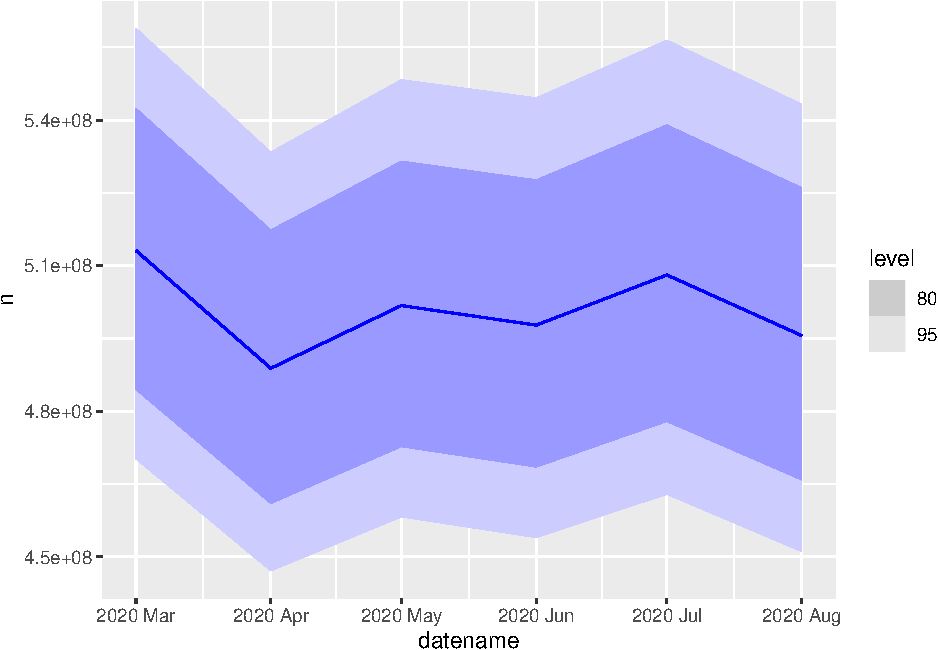
\includegraphics{paper_files/figure-latex/all-prescribing-modelling-1.pdf}

\begin{figure}
\centering
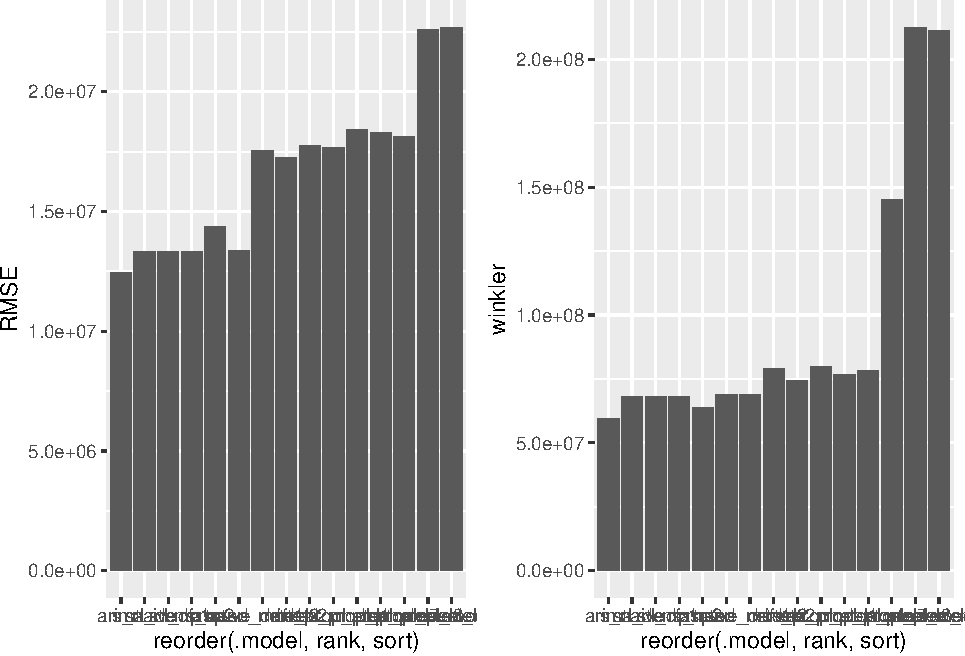
\includegraphics{paper_files/figure-latex/all-prescribing-model-accuracy-hist-1.pdf}
\caption{\label{fig:all-prescribing-model-accuracy-hist}All prescribing, model accuracy}
\end{figure}

\begin{verbatim}
## Warning: Removed 108 row(s) containing missing values (geom_path).
\end{verbatim}

\begin{figure}
\centering
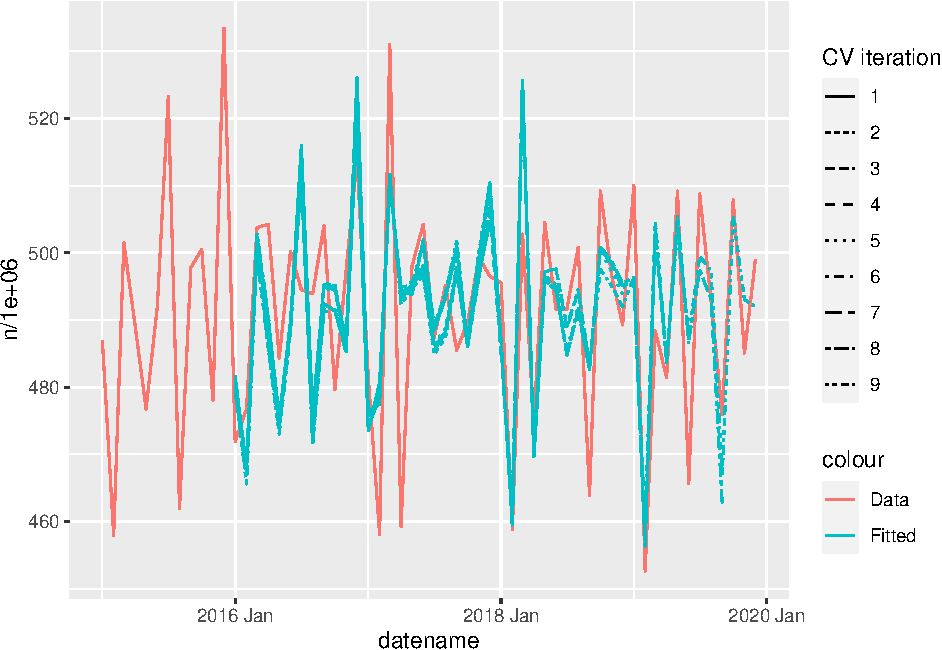
\includegraphics{paper_files/figure-latex/all-prescribing-cv-plot-1.pdf}
\caption{\label{fig:all-prescribing-cv-plot}All prescribing, best model CV fit}
\end{figure}

\begin{verbatim}
## Warning: Ignoring unknown aesthetics: fill

## Warning: Ignoring unknown aesthetics: fill

## Warning: Ignoring unknown aesthetics: fill
\end{verbatim}

\begin{verbatim}
## Warning: Removed 12 row(s) containing missing values (geom_path).
\end{verbatim}

\begin{figure}
\centering
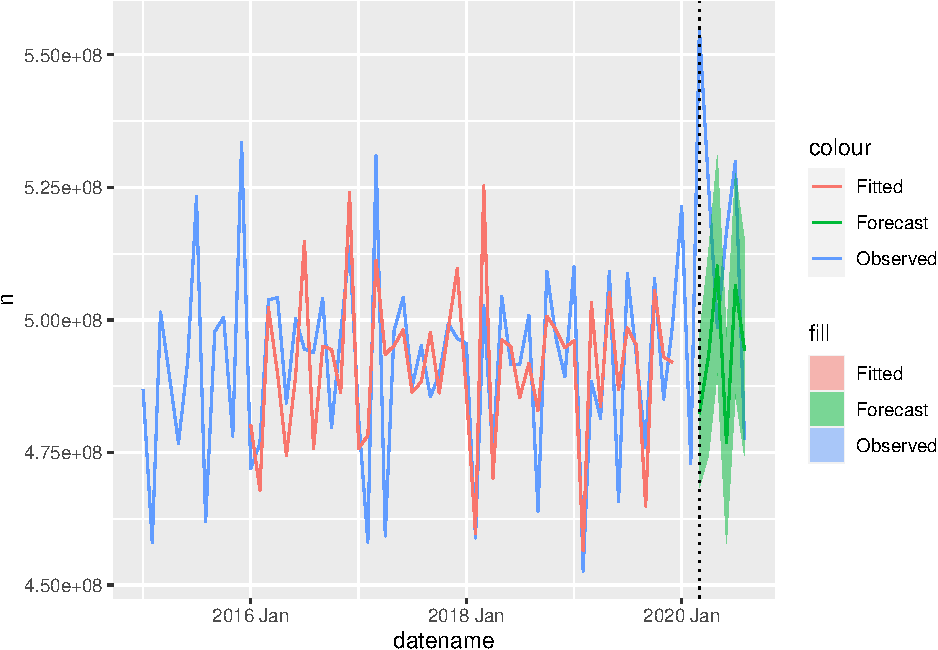
\includegraphics{paper_files/figure-latex/all-prescribing-forecast-plot-1.pdf}
\caption{\label{fig:all-prescribing-forecast-plot}All prescribing, best model fit and forecast}
\end{figure}

\begin{figure}
\centering
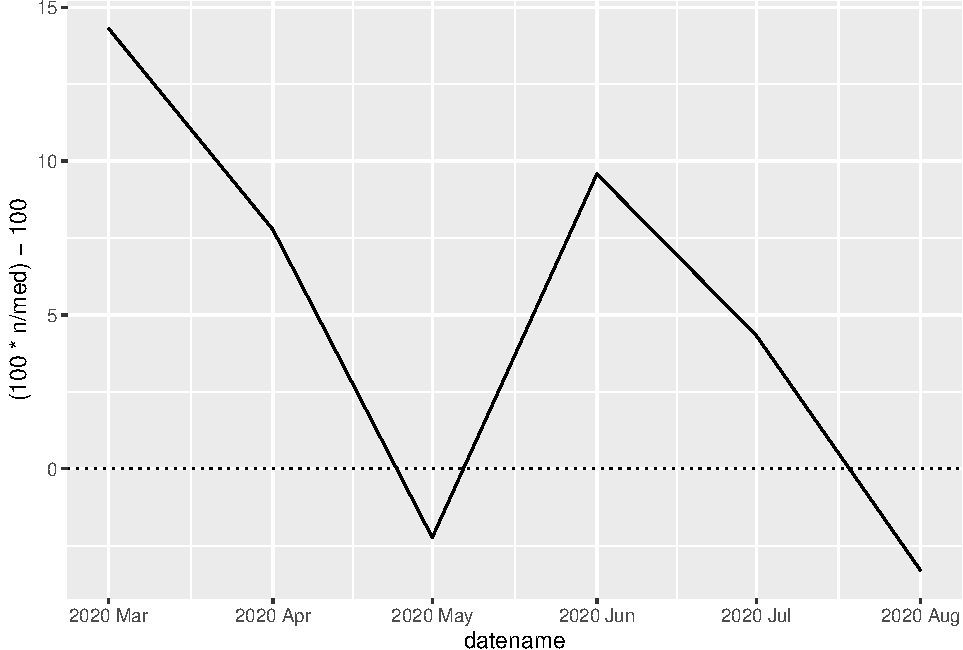
\includegraphics{paper_files/figure-latex/all-prescribing-pct-change-plot-1.pdf}
\caption{\label{fig:all-prescribing-pct-change-plot}Percentage difference in all prescribing}
\end{figure}

\hypertarget{specific-drugs}{%
\subsubsection{Specific drugs}\label{specific-drugs}}

\hypertarget{discussion}{%
\section{Discussion}\label{discussion}}

\newpage

\hypertarget{references}{%
\section{References}\label{references}}

\begingroup
\setlength{\parindent}{-0.5in}
\setlength{\leftskip}{0.5in}

\hypertarget{refs}{}
\leavevmode\hypertarget{ref-R-papaja}{}%
Aust, F., \& Barth, M. (2020). \emph{papaja: Create APA manuscripts with R Markdown}. \url{https://github.com/crsh/papaja}

\leavevmode\hypertarget{ref-R-future}{}%
Bengtsson, H. (2020). \emph{A unifying framework for parallel and distributed processing in r using futures}. \url{https://arxiv.org/abs/2008.00553}

\leavevmode\hypertarget{ref-Box2015}{}%
Box, G. E. P., Jenkins, G. M., Reinsel, G. C. .., \& Ljung, G. M. (2015). \emph{Time series analysis: forecasting and control} (5th ed.). John Wiley \& Sons.

\leavevmode\hypertarget{ref-Chatfield1978}{}%
Chatfield, C. (1978). The Holt-Winters Forecasting Procedure. \emph{Journal of the Royal Statistical Society: Series C (Applied Statistics)}, \emph{27}(3), 264--279.

\leavevmode\hypertarget{ref-R-rebus}{}%
Cotton, R. (2017). \emph{Rebus: Build regular expressions in a human readable way}. \url{https://CRAN.R-project.org/package=rebus}

\leavevmode\hypertarget{ref-R-Rcpp_b}{}%
Eddelbuettel, D., \& Balamuta, J. J. (2018). Extending extitR with extitC++: A Brief Introduction to extitRcpp. \emph{The American Statistician}, \emph{72}(1), 28--36. \url{https://doi.org/10.1080/00031305.2017.1375990}

\leavevmode\hypertarget{ref-R-Rcpp_a}{}%
Eddelbuettel, D., \& François, R. (2011). Rcpp: Seamless R and C++ integration. \emph{Journal of Statistical Software}, \emph{40}(8), 1--18. \url{https://doi.org/10.18637/jss.v040.i08}

\leavevmode\hypertarget{ref-R-lubridate}{}%
Grolemund, G., \& Wickham, H. (2011). Dates and times made easy with lubridate. \emph{Journal of Statistical Software}, \emph{40}(3), 1--25. \url{https://www.jstatsoft.org/v40/i03/}

\leavevmode\hypertarget{ref-R-MplusAutomation}{}%
Hallquist, M. N., \& Wiley, J. F. (2018). MplusAutomation: An R package for facilitating large-scale latent variable analyses in Mplus. \emph{Structural Equation Modeling}, 1--18. \url{https://doi.org/10.1080/10705511.2017.1402334}

\leavevmode\hypertarget{ref-R-purrr}{}%
Henry, L., \& Wickham, H. (2020a). \emph{Purrr: Functional programming tools}. \url{https://CRAN.R-project.org/package=purrr}

\leavevmode\hypertarget{ref-R-rlang}{}%
Henry, L., \& Wickham, H. (2020b). \emph{Rlang: Functions for base types and core r and 'tidyverse' features}. \url{https://CRAN.R-project.org/package=rlang}

\leavevmode\hypertarget{ref-Marsh2009}{}%
Marsh, H. W., Muthén, B. O., Asparouhov, T., Lüdtke, O., Robitzsch, A., Morin, A. J. S., \& Trautwein, U. (2009). \emph{Exploratory structural equation modeling, integrating CFA and EFA: Application to students' evaluations of university teaching} (Vol. 16, pp. 439--476). \url{https://doi.org/10.1080/10705510903008220}

\leavevmode\hypertarget{ref-McLachlan2000}{}%
McLachlan, G., \& Peel, D. (2000). \emph{Finite mixture models}. Wiley.

\leavevmode\hypertarget{ref-R-tibble}{}%
Müller, K., \& Wickham, H. (2021). \emph{Tibble: Simple data frames}. \url{https://CRAN.R-project.org/package=tibble}

\leavevmode\hypertarget{ref-Nylund2007}{}%
Nylund, K. L., Asparouhov, T., \& Muthén, B. O. (2007). Deciding on the number of classes in latent class analysis and growth mixture modeling: A Monte Carlo simulation study. \emph{Structural Equation Modeling}, \emph{14}(4), 535--569. \url{https://doi.org/10.1080/10705510701575396}

\leavevmode\hypertarget{ref-R-fable.prophet}{}%
O'Hara-Wild, M. (2020). \emph{Fable.prophet: Prophet modelling interface for 'fable'}. \url{https://CRAN.R-project.org/package=fable.prophet}

\leavevmode\hypertarget{ref-R-fasster}{}%
O'Hara-Wild, M., \& Hyndman, R. (2021). \emph{Fasster: Fast additive switching of seasonality, trend and exogenous regressors}. \url{https://github.com/mitchelloharawild/fasster}

\leavevmode\hypertarget{ref-R-fable}{}%
O'Hara-Wild, M., Hyndman, R., \& Wang, E. (2021a). \emph{Fable: Forecasting models for tidy time series}. \url{https://CRAN.R-project.org/package=fable}

\leavevmode\hypertarget{ref-R-fabletools}{}%
O'Hara-Wild, M., Hyndman, R., \& Wang, E. (2021b). \emph{Fabletools: Core tools for packages in the 'fable' framework}. \url{https://CRAN.R-project.org/package=fabletools}

\leavevmode\hypertarget{ref-R-feasts}{}%
O'Hara-Wild, M., Hyndman, R., \& Wang, E. (2021c). \emph{Feasts: Feature extraction and statistics for time series}. \url{https://CRAN.R-project.org/package=feasts}

\leavevmode\hypertarget{ref-R-base}{}%
R Core Team. (2020). \emph{R: A language and environment for statistical computing}. R Foundation for Statistical Computing. \url{https://www.R-project.org/}

\leavevmode\hypertarget{ref-R-tidyLPA}{}%
Rosenberg, J. M., Beymer, P. N., Anderson, D. J., Van Lissa, C. J., \& Schmidt, J. A. (2018). TidyLPA: An r package to easily carry out latent profile analysis (lpa) using open-source or commercial software. \emph{Journal of Open Source Software}, \emph{3}(30), 978. \url{https://doi.org/10.21105/joss.00978}

\leavevmode\hypertarget{ref-Schwartz1978}{}%
Schwartz, G. (1978). Estimating the dimesion of a model. \emph{The Annals of Statistics1}, \emph{6}(2), 461--464.

\leavevmode\hypertarget{ref-R-rstan}{}%
Stan Development Team. (2020a). \emph{RStan: The R interface to Stan}. \url{http://mc-stan.org/}

\leavevmode\hypertarget{ref-R-StanHeaders}{}%
Stan Development Team. (2020b). \emph{StanHeaders: Headers for the R interface to Stan}. \url{https://mc-stan.org/}

\leavevmode\hypertarget{ref-Taylor2018}{}%
Taylor, S. J., \& Letham, B. (2018). Forecasting at Scale. \emph{American Statistician}, \emph{72}(1), 37--45. \url{https://doi.org/10.1080/00031305.2017.1380080}

\leavevmode\hypertarget{ref-R-prophet}{}%
Taylor, S., \& Letham, B. (2020). \emph{Prophet: Automatic forecasting procedure}. \url{https://CRAN.R-project.org/package=prophet}

\leavevmode\hypertarget{ref-Thomson2019}{}%
Thomson, M. E., Pollock, A. C., Önkal, D., \& Gönül, M. S. (2019). Combining forecasts: Performance and coherence. \emph{International Journal of Forecasting}, \emph{35}(2), 474--484. \url{https://doi.org/10.1016/j.ijforecast.2018.10.006}

\leavevmode\hypertarget{ref-R-furrr}{}%
Vaughan, D., \& Dancho, M. (2021). \emph{Furrr: Apply mapping functions in parallel using futures}. \url{https://CRAN.R-project.org/package=furrr}

\leavevmode\hypertarget{ref-R-tsibble}{}%
Wang, E., Cook, D., \& Hyndman, R. J. (2020). A new tidy data structure to support exploration and modeling of temporal data. \emph{Journal of Computational and Graphical Statistics}, \emph{29}(3), 466--478. \url{https://doi.org/10.1080/10618600.2019.1695624}

\leavevmode\hypertarget{ref-R-ggplot2}{}%
Wickham, H. (2016). \emph{Ggplot2: Elegant graphics for data analysis}. Springer-Verlag New York. \url{https://ggplot2.tidyverse.org}

\leavevmode\hypertarget{ref-R-stringr}{}%
Wickham, H. (2019). \emph{Stringr: Simple, consistent wrappers for common string operations}. \url{https://CRAN.R-project.org/package=stringr}

\leavevmode\hypertarget{ref-R-tidyr}{}%
Wickham, H. (2020). \emph{Tidyr: Tidy messy data}. \url{https://CRAN.R-project.org/package=tidyr}

\leavevmode\hypertarget{ref-R-forcats}{}%
Wickham, H. (2021). \emph{Forcats: Tools for working with categorical variables (factors)}. \url{https://CRAN.R-project.org/package=forcats}

\leavevmode\hypertarget{ref-R-tidyverse}{}%
Wickham, H., Averick, M., Bryan, J., Chang, W., McGowan, L. D., François, R., Grolemund, G., Hayes, A., Henry, L., Hester, J., Kuhn, M., Pedersen, T. L., Miller, E., Bache, S. M., Müller, K., Ooms, J., Robinson, D., Seidel, D. P., Spinu, V., \ldots{} Yutani, H. (2019). Welcome to the tidyverse. \emph{Journal of Open Source Software}, \emph{4}(43), 1686. \url{https://doi.org/10.21105/joss.01686}

\leavevmode\hypertarget{ref-R-dplyr}{}%
Wickham, H., François, R., Henry, L., \& Müller, K. (2021). \emph{Dplyr: A grammar of data manipulation}. \url{https://CRAN.R-project.org/package=dplyr}

\leavevmode\hypertarget{ref-R-readr}{}%
Wickham, H., \& Hester, J. (2020). \emph{Readr: Read rectangular text data}. \url{https://CRAN.R-project.org/package=readr}

\leavevmode\hypertarget{ref-R-serCymruTools}{}%
Will, H. (2021). \emph{SerCymruTools: Tools for analysing gp prescribing data}.

\endgroup

\end{document}
